\chapter{Figures and Tables}
\begin{figure}[H]
    \centering
    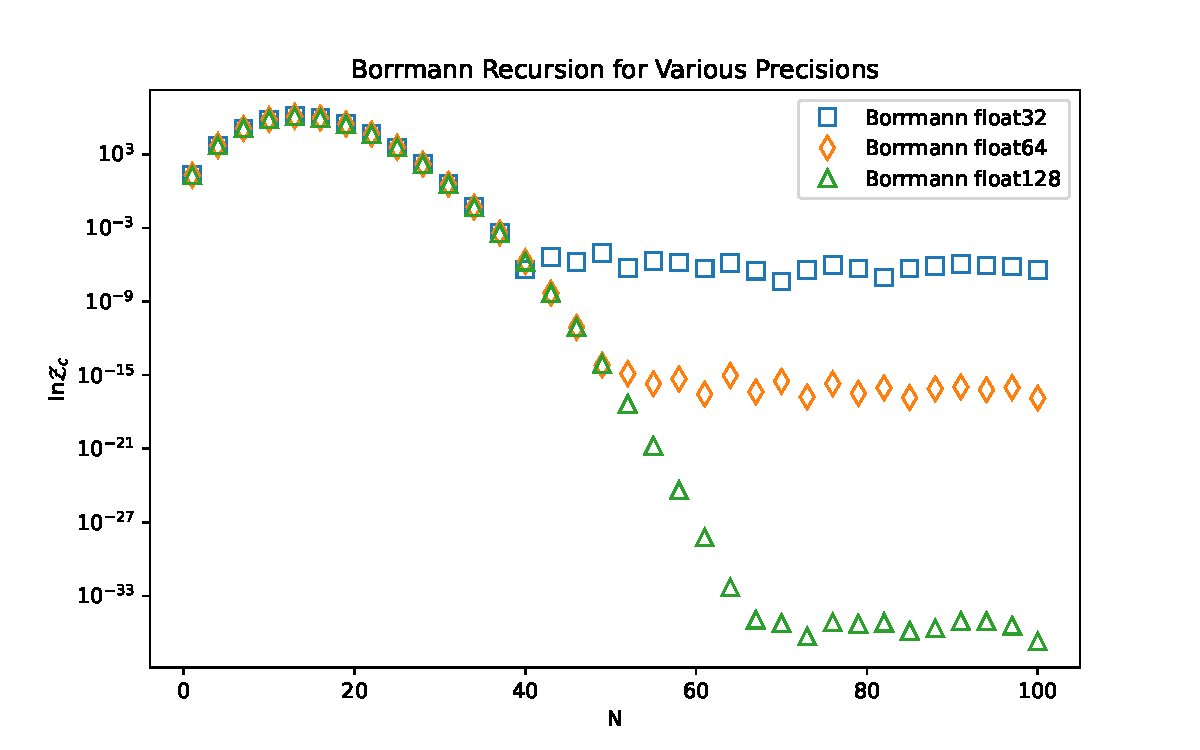
\includegraphics[scale=0.6]{figures/pdf/Borrmann accuracy.pdf}
    \caption{The solution for the Borrman recursive relation of the canonical partition function for different machine precisions. As $N$ increases, the required precision to accurately find the partition function also increases. The breakdown of the recursion is only delayed by the precision used. Therefore, this is numerically expensive to calculate for $N>60$. Figure adapted from \cite{Jiang}.}
    \label{fig:BorrmannAcc}
\end{figure}
\begin{figure}[H]
    \centering
    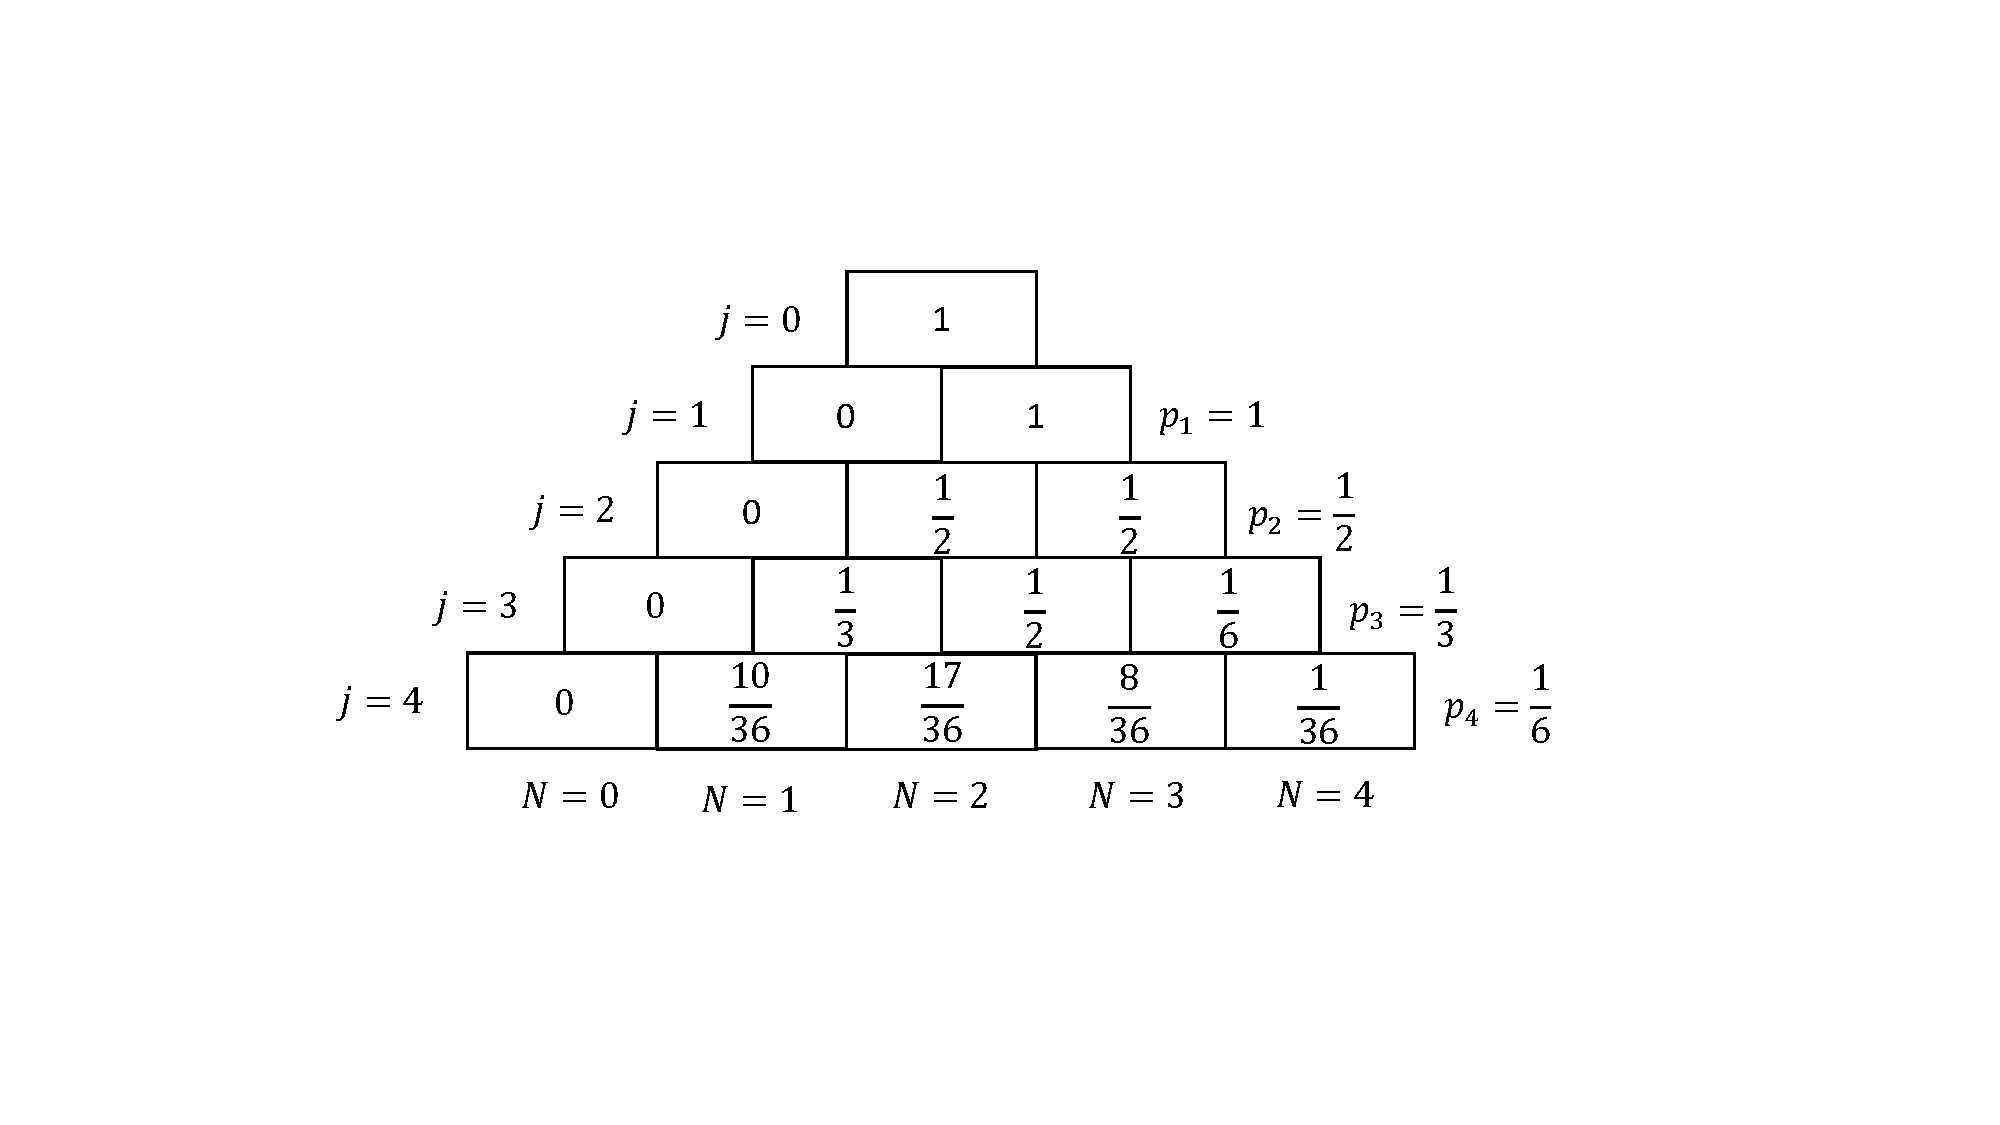
\includegraphics[scale=0.55]{figures/pdf/PBTriangle.pdf}
    \caption{The Poisson binomial triangle for the example considered above. After using the recurrence relation to include all probability levels, the base of the triangle gives the particle number distribution for the system.}
    \label{fig:Poisson Binomial Triangle}
\end{figure}
\begin{figure}[H]
    \centering
    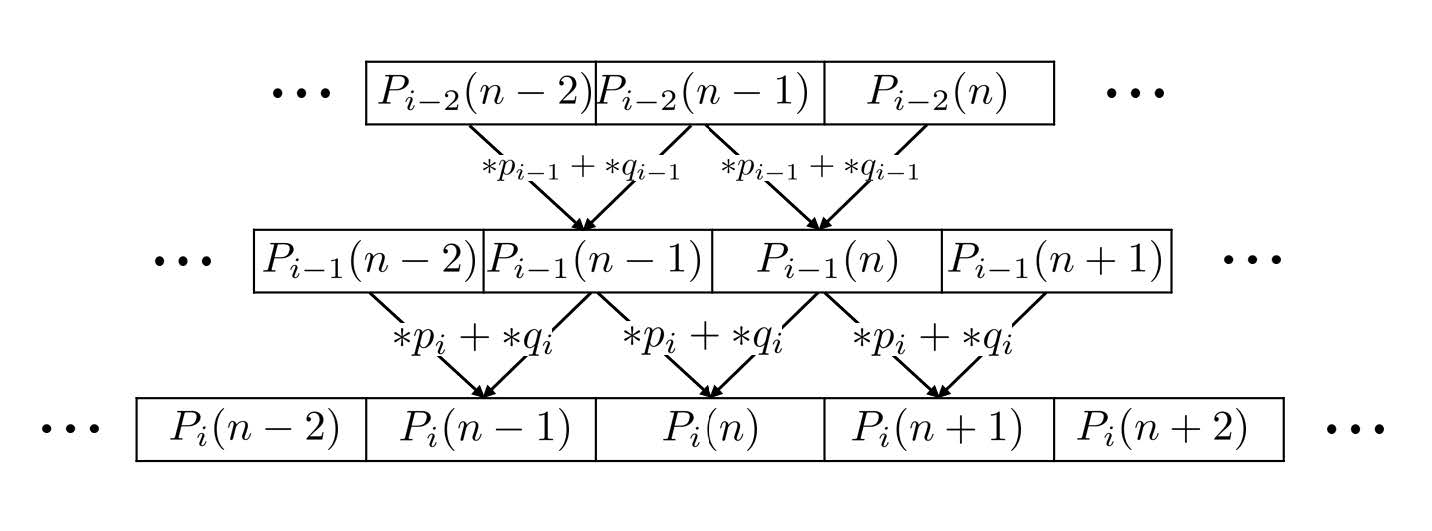
\includegraphics[scale=0.8]{figures/pdf/PBrecursion.jpg}
    \caption{The generalized Pascal triangle. Here, $i=j$ denotes the number of probabilites included from the distribution, $p$ denotes the probabilities, and $q$ denotes the complimentary probability. $P_i(n)$ is term $n$ in the probability distribution that contains $i$ of the probabilities. Each new term is the sum of the arrows pointing to it. Each arrow is multiplied ($*$) by $p_i$ or $q_i$.}
    \label{fig:General Poisson Binomial Recursion}
\end{figure}
\begin{figure}[H]
    \centering
    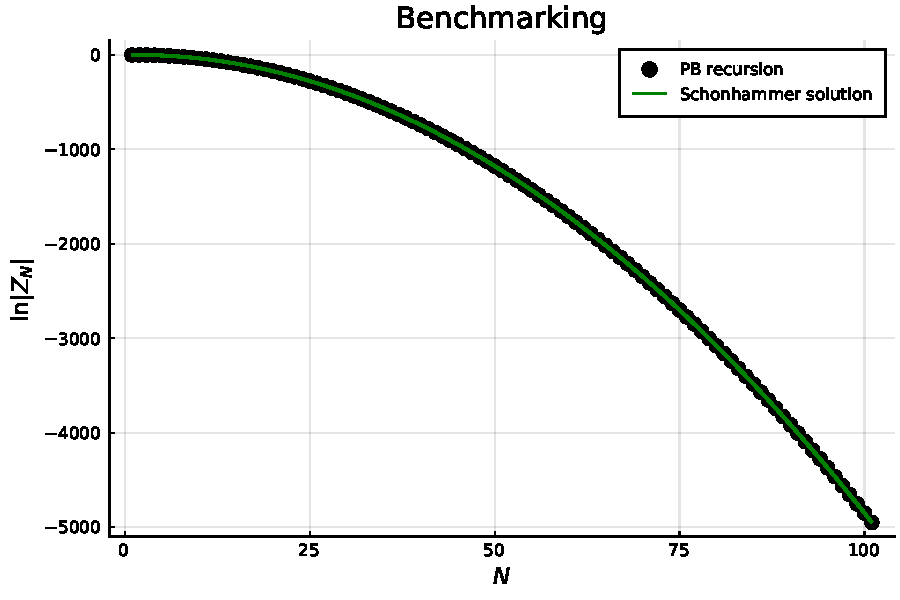
\includegraphics[scale=0.75]{figures/pdf/Benchmarking.pdf}
    \caption{Solution from Poisson Binomial recursive method versus the exact solution for the 1D simple harmonic oscillator. The black circles are the solutions from the Poisson Binomial recursion method. The green line is the exact solution using Sch\"onhammer's Eq.(\ref{schoneqn})}
    \label{fig: schon solution}
\end{figure}
\begin{figure}[H]
    \centering
    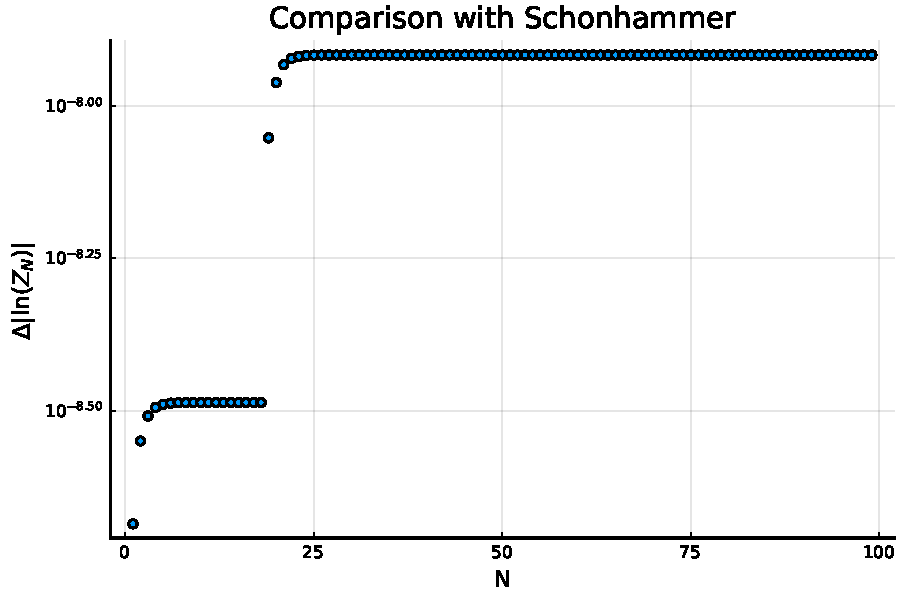
\includegraphics[scale=0.75]{figures/pdf/Benchdiff.pdf}
    \caption{The difference between the solutions presented in Fig. (\ref{fig: schon solution}). The precision of the Poisson binomial method was set to $10^{-8}$ which controls the range of the y-axis. The jump in error is due to the exclusion of terms below the Fermi level. Terms are chosen to be excluded if their occupation probability differs from one by a chosen cutoff value. In this case they are assumed to be in an occupied state. }
    \label{fig: schon diff}
\end{figure}
\begin{figure}[H]
    \centering
    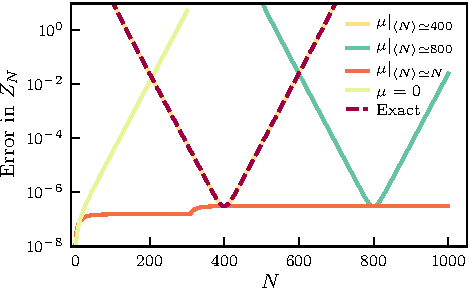
\includegraphics[scale=1.4]{figures/pdf/Plot1.pdf}
    \caption{The error associated with keeping the chemical potential $\mu$ fixed for a range of $N$ particles values. The accuracy of $\mu|_N$ is at the minimum error in a small range around $N$. The further $N$ is away from $\mu|_N$, the larger the error becomes. Therefore, it's necessary to recalculated $\mu$ for each value of $N$ in order to keep the error of the canonical partition function $Z_N$ to a minimum. This figure was provided by Jiangyong Yu. }
    \label{fig:Errors}
\end{figure}
\begin{figure}[H]
    \centering
    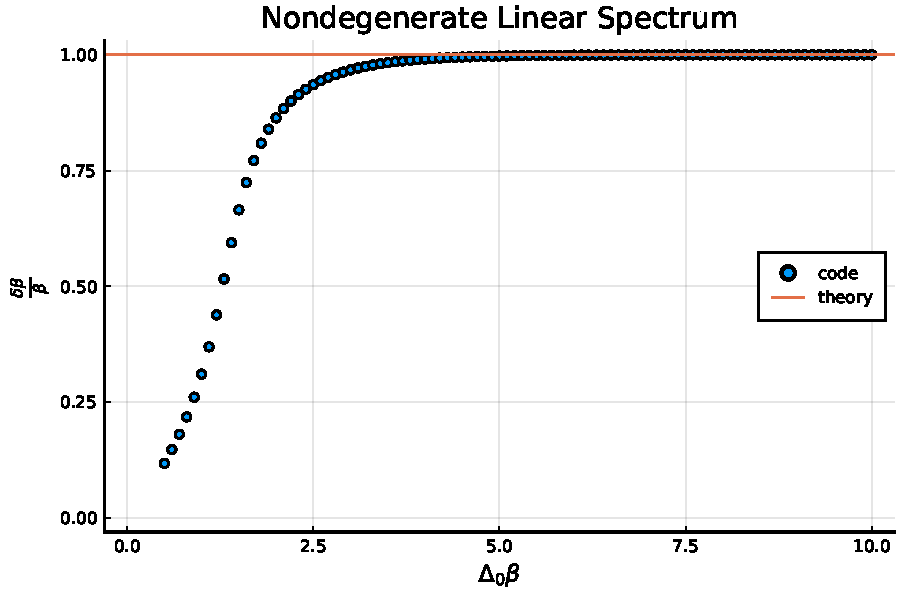
\includegraphics[scale=.75]{figures/pdf/linE_nondeg_N10.pdf}
    \caption{Error in $\beta^*$ measurement for a nondegenerate linear energy spectrum. Once $\Delta_0\beta$ is large enough, the error calculated from the code increases to $100\%$ as expected from the theory. }
    \label{fig:linnondeg}
\end{figure}
\begin{figure}[H]
    \centering
    \includegraphics[scale=0.75]{figures/pdf/quadE_nondeg_N10_Δ0=6.333.pdf}
    \caption{Error in $\beta^*$ measurement for a nondegenerate quadratic energy spectrum. Once $\Delta_0\beta$ is large enough, the error calculated from the code increases to $100\%$ as expected from the theory. }
    \label{fig:quadnondeg}
\end{figure}
\begin{figure}[H]
    \centering
    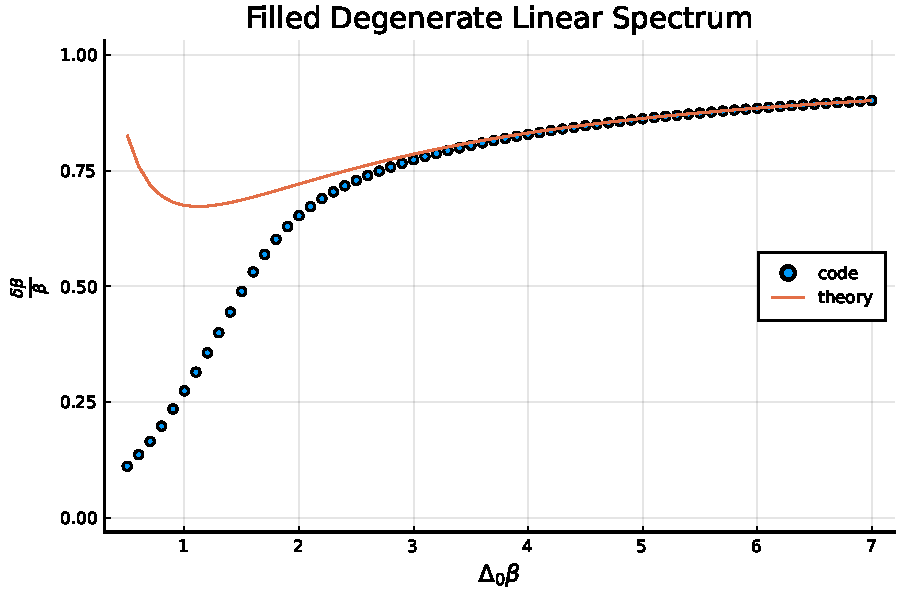
\includegraphics[scale=0.75]{figures/pdf/linE_filldegen_g0-2_N10.pdf}
    \caption{Error in $\beta^*$ measurement for a linear energy spectrum with a filled degenerate Fermi level. Once $\Delta_0\beta$ is large enough, the error calculated from the code follows the theoretical line in orange.}
    \label{fig:Filled}
\end{figure}
\begin{figure}[H]
    \centering
    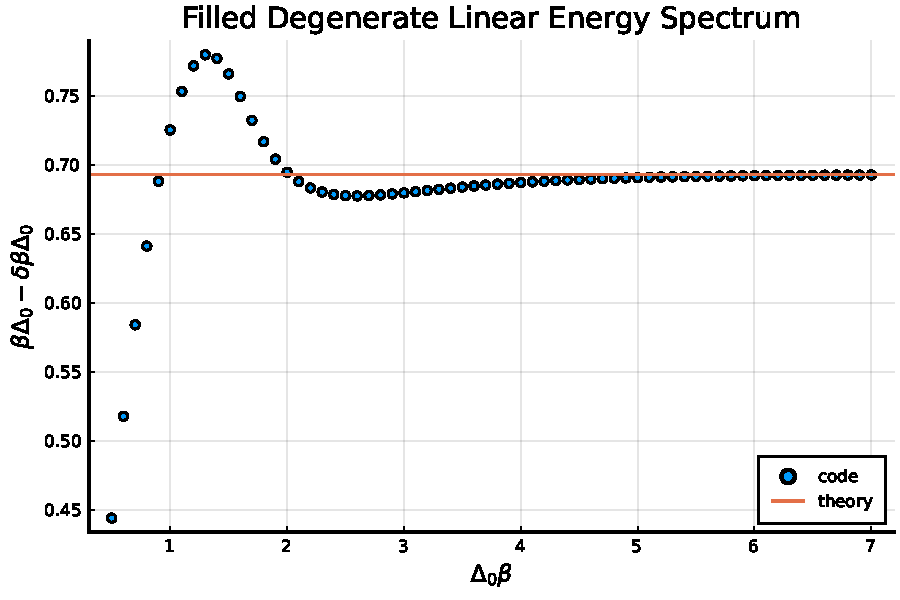
\includegraphics[scale=0.75]{figures/pdf/linE_filldegen_g0-2_N10_1.pdf}
    \caption{Error in $\beta^*$ measurement for a linear energy spectrum with a filled
degenerate Fermi level. The figure is adjusted to plot Eq.\@ (\ref{3.2}). Once $\Delta_0\beta$ is large enough, the $\ln(g_0g_1)$ limit is reached. For the case shown above, $g_0=2$ and $g_1=1$ so the asymptotic limit is $\ln(2)$ as shown in orange.}
    \label{fig:FilledDegenerateLinearSpectrumAdjustedError}
\end{figure}
\begin{figure}[H]
    \centering
    \includegraphics[scale=0.75]{figures/pdf/quadE_filldegen_g0-2_N10_Δ0-7.pdf}
    \caption{Error in $\beta^*$ measurement for a quadratic energy spectrum with a filled
degenerate Fermi level. Once the temperature is small enough, the error calculated from the code
follows the theoretical line in orange.}
    \label{fig:FilledDegenerate}
\end{figure}
\begin{figure}[H]
    \centering
    \includegraphics[scale=0.75]{figures/pdf/quadE_filldegen_g0-2_N10_Δ0-7_1.pdf}
    \caption{Error in $\beta^*$ measurement for a quadratic energy spectrum with a filled
degenerate Fermi level. The figure is adjusted to plot Eq.\@ (\ref{3.2}). Once $\Delta_0\beta$ is large enough, the $\ln(g_0g_1)$ limit is reached. For the case shown above, $g_0=2$ and $g_1=1$ so the asymptotic limit is $\ln(2)$ as shown in orange.}
    \label{fig:FilledDegenerate2}
\end{figure}
\begin{figure}[H]
    \centering
    \includegraphics[scale=0.75]{figures/pdf/linE_partfilldegen_N9_g0-2_l-1_Δ0-1.pdf}
    \caption{Error in $\beta^*$ measurement for a linear energy spectrum with a partially filled Fermi level. Once $\Delta_0\beta$ is large enough, the error calculated from the code follows the theoretical line in orange.}
    \label{fig:PartiallyFilledDegenerateLinearSpectrum}
\end{figure}
\begin{figure}[H]
    \centering
    \includegraphics[scale=0.75]{figures/pdf/linE_partfilldegen_N9_g0-2_l-1_Δ0-1_1.pdf}
    \caption{Error in $\beta^*$ measurement for a linear energy spectrum with a partially filled Fermi level. The figure is adjusted to plot Eq.\@ (\ref{3.3}). Once $\Delta_0\beta$ is large enough, the error calculated from the code follows the theoretical line in orange.}
    \label{fig:PartiallyFilledDegenerateLinearSpectrumAdjustedError}
\end{figure}
\begin{figure}[H]
    \centering
    \includegraphics[scale=0.75]{figures/pdf/quadE_partfilldegen_g0-2_l-1_N9_Δ0-7.pdf}
    \caption{Error in $\beta^*$ measurement for a quadratic energy spectrum with a partially filled Fermi level. Once $\Delta_0\beta$ is large enough, the error calculated from the code follows the theoretical line in orange.}
    \label{fig:PartiallyFilledDegenerateQuadraticSpectrumError}
\end{figure}
\begin{figure}[H]
    \centering
    \includegraphics[scale=0.75]{figures/pdf/quadE_partfilldegen_g0-2_l-1_N9_Δ0-7_1.pdf}
    \caption{Error in $\beta^*$ measurement for a quadratic energy spectrum with a partially filled Fermi level. The figure is adjusted to plot Eq.\@ (\ref{3.3}). Once $\Delta_0\beta$ is large enough, the error calculated from the code follows the theoretical line in orange.}
    \label{fig:PartiallyFilledDegenerateQuadraticSpectrumAdjustedError}
\end{figure}
\begin{figure}[H]
    \centering
    \includegraphics[scale=0.75]{figures/pdf/linE_almostdegen_nondegen_g0-2_l-1_N10_Δ0-1.pdf}
    \caption{Error in $\beta^*$ measurement of a linear energy spectrum with an Fermi level that is almost degenerate. The error follows the partially filled degenerate Fermi level case shown in green until the $\Delta_0 \beta$ is large enough to break the degeneracy and return to the non-degenerate theory shown in purple.}
    \label{fig:linE_almostdegen}
\end{figure}
\begin{figure}[H]
    \centering
    \includegraphics[scale=0.75]{figures/pdf/quadE_almostdegen_nondegen_g0-2_l-1_N10_Δ0-6.333.pdf}
    \caption{Error in $\beta^*$ measurement of a quadratic energy spectrum with an Fermi level that is almost degenerate. The error follows the partially filled degenerate Fermi level case shown in green until the $\Delta_0 \beta$ is large enough to break the degeneracy and return to the non-degenerate theory shown in purple.}
    \label{fig:quadE_almostdegen}
\end{figure}
\begin{table}[H]
    \centering
    \caption{Experimental results of cold atom experiments.}
    \label{tab:experiment}
    \begin{tabular}{||c c c||}
           \hline
         & Mukherjee et al.\@ \cite{Mukherjee2017} & Hueck et al.\@ \cite{Hueck2018} \\ [0.5ex]
         \hline
         $\frac{E_F}{k_B}$ & $6.213\times10^{-7}$K & $1.498\times10^{-7}$K\\ 
         \hline
         $\frac{T}{T_F}$ & 0.16 & 0.14 \\
         \hline
         $\frac{\Delta}{k_B}$ & $5.73\times 10^{-9}$K & $1.05\times 10^{-9}$K\\
         \hline
         $\Delta\beta$ & 0.058 & 0.052 \\ [1ex]
         \hline
    \end{tabular}
\end{table}
\begin{figure}[H]
    \centering
    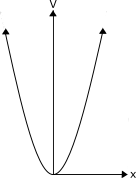
\includegraphics{figures/pdf/SHOpot.png}
    \caption{Simple Harmonic Potential. Increases quadratically as $x$ moves away from 0.}
    \label{fig:SHOpot}
\end{figure}
\begin{figure}[H]
    \centering
    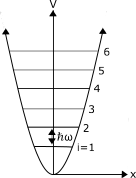
\includegraphics[scale=1.0]{figures/pdf/SHOspectrum.png}
    \caption{The energy spectrum of the simple harmonic oscillator. The spacing between energy levels is a constant $\hbar\omega$. For this reason it is called a linear spectrum.}
    \label{fig:Simple Harmonic Oscillator Spectrum}
\end{figure}
\begin{figure}[H]
    \centering
    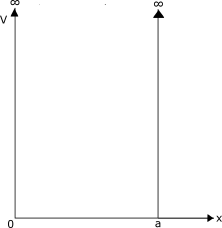
\includegraphics[scale=0.75]{figures/pdf/sqwellpot.png}
    \caption{Infinite Well Potential. This potential is zero between two endpoints and infinite everywhere else.}
    \label{fig: Infinite Well Potential}
\end{figure}
\begin{figure}[H]
    \centering
    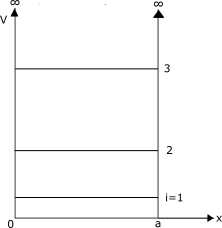
\includegraphics[scale=1.0]{figures/pdf/sqwellspec.png}
    \caption{Energy spectrum of the infinite square well. The distance between levels increases linearly. For this reason it is called a quadratic spectrum}
    \label{fig:Energy spectrum of the infinite square well}
\end{figure}
